\chapter{Local Flatness, Parallel Transport, and Curvature}

\lectureoverview{The equivalence principle lets us remove gravity at one
event, but not throughout a region containing tidal forces. We will make
that statement precise in two stages. First we use coordinate freedom to
set the first derivatives of the metric, and hence the connection, to zero
at one point. Then we transport vectors around closed curves and discover
the obstruction to extending that local flattening: curvature.}

\section{Proper Time in Space-Time}

There are two objectives for this lecture. We want to understand geodesics
more fully, and we want to connect geodesic motion with gravitational
force. Both objectives require us to work in space-time rather than space
alone.

Space-time has a metric just as an ordinary geometric space does. Greek
indices run over the four coordinates,
\begin{equation}
  \mu,\nu=0,1,2,3,
\end{equation}
with \(0\) denoting time and \(1,2,3\) denoting space. Along a timelike
worldline, the invariant interval is the proper time:
\begin{equation}
  d\tau^2=g_{\mu\nu}\,dx^\mu dx^\nu.
  \label{eq:l06-proper-time}
\end{equation}
In an inertial frame of special relativity and in units \(c=1\),
\begin{equation}
  \eta_{\mu\nu}
  =
  \operatorname{diag}(1,-1,-1,-1),
  \qquad
  d\tau^2=dt^2-dx^2-dy^2-dz^2.
  \label{eq:l06-minkowski}
\end{equation}
If \(\tau\) and \(t\) are measured in units of time while the spatial
coordinates retain units of length, restoring the speed of light gives
\begin{equation}
  d\tau^2
  =
  dt^2-\frac{dx^2+dy^2+dz^2}{c^2}.
  \label{eq:l06-c-restored}
\end{equation}

\begin{figure}[tbp]
  \centering
  
\includegraphics[width=0.88\textwidth]{lecture_06_figure_01.png}
  \caption{The proper-time interval, the Minkowski metric with signature
  \((+---)\), and the component form of the interval.}
  \lectureframe{00:04:00}
\end{figure}

For a particle with ordinary speed \(v\),
\begin{equation}
  d\tau
  =
  dt\sqrt{1-\frac{v^2}{c^2}}.
  \label{eq:l06-time-dilation}
\end{equation}
When \(v\ll c\), proper time and coordinate time are nearly equal. More
generally, \(d\tau\) is what a clock carried by the particle records. The
coordinate \(t\) is a label assigned by the chosen frame.

\begin{classroomqa}
\audiencequestion{Does a clock moving with the object record \(dt\), or
does it record \(d\tau\)?
\lecturetimestamp{00:06:57--00:08:02}}
\lecturerresponse{It records \(d\tau\). A tape measure laid along a curve
records distance along that curve rather than either Cartesian coordinate.
In the same way, the moving clock is a space-time tape measure: its ticks
mark proper time along the worldline.}
\end{classroomqa}

The formal apparatus is now familiar. The metric, covariant and
contravariant tensors, Christoffel symbols, and covariant derivatives are
constructed in space-time exactly as in ordinary space. The essential
difference is the Lorentzian signature: one direction has the opposite
sign from the other three.

\begin{classroomqa}
\audiencequestion{Does enlarging the metric from four dimensions to five
or more account for the extra dimensions discussed in string theory?
\lecturetimestamp{00:09:38--00:10:22}}
\lecturerresponse{The dimension is exactly the number of independent
coordinates and therefore the size of the metric matrix. This statement
is not peculiar to string theory; the tensor rules have the same form in
any dimension. A particular theory must still explain why those
dimensions are present and what geometry they possess.}
\end{classroomqa}

\section{Accelerated Coordinates Are Not Yet Curvature}

In flat space-time we can always use inertial Cartesian coordinates, so
curved coordinates may look like an unnecessary complication. They become
useful when the observer is accelerated. Relative to inertial
\((T,X)\)-coordinates, the coordinate lines of a uniformly accelerated
family are hyperbolic. A freely moving body follows a straight worldline
in the inertial chart but appears accelerated in the curved chart.

\begin{figure}[tbp]
  \centering
  
\includegraphics[width=0.84\textwidth]{lecture_06_figure_02.png}
  \caption{Straight inertial axes and a family of curved accelerated
  coordinate lines. A straight inertial worldline acquires coordinate
  acceleration in the accelerated description.}
  \lectureframe{00:12:18}
\end{figure}

This is the elevator lesson behind the equivalence principle. An
accelerated frame produces an apparent gravitational field. Conversely,
inside a freely falling laboratory, a nearly uniform gravitational field
can be removed locally. Curved coordinates can therefore imitate gravity.
They do not, by themselves, imply that space-time is curved.

The word \emph{locally} is decisive. Near a star, different parts of a
large elevator accelerate by slightly different amounts and directions.
Those relative accelerations are tidal effects. By shrinking the elevator
we can make them arbitrarily small at one event, but no single accelerated
coordinate system removes the field throughout an extended region. The
mathematical obstruction to doing so is curvature.

\section{Global Flatness and Local Inertial Coordinates}

A space is flat if there exists a coordinate system in which the metric
components are constant throughout the region:
\begin{equation}
  \partial_r g_{mn}=0
  \qquad
  \text{everywhere in the region}.
  \label{eq:l06-global-flatness}
\end{equation}
The constant matrix need not literally be \(\delta_{mn}\). Uniform
oblique coordinates produce constant off-diagonal entries. A further
linear change of basis can put a positive-definite metric into Euclidean
form, or a Lorentzian metric into Minkowski form.

\begin{figure}[tbp]
  \centering
  
\includegraphics[width=0.86\textwidth]{lecture_06_figure_03.png}
  \caption{Flatness expressed by coordinates in which the first
  derivatives of the metric vanish everywhere. The same condition can
  always be achieved at one regular point even when the geometry is
  curved.}
  \lectureframe{00:19:32}
\end{figure}

Curved geometry does not permit Eq.~\eqref{eq:l06-global-flatness}
throughout a neighborhood, but smooth coordinate freedom always permits
the pointwise conditions
\begin{equation}
  g_{mn}(p)=\delta_{mn},
  \qquad
  \partial_r g_{mn}(p)=0
  \label{eq:l06-normal-spatial}
\end{equation}
in a Riemannian space. In space-time, \(\delta_{mn}\) is replaced by
\(\eta_{\mu\nu}\). These are normal coordinates, or local inertial
coordinates in the Lorentzian case. They flatten the metric through first
order at \(p\), not across a finite region.

\section{Counting the Coordinate Freedom}

The lecture's local argument begins after a linear transformation has
already aligned and normalized the metric at \(p\). Put the common origin
at \(x=0=y\), and consider a quadratic change of coordinates,
\begin{equation}
  y^m
  =
  x^m+C^m{}_{rs}x^r x^s+O(x^3).
  \label{eq:l06-quadratic-map}
\end{equation}
Only the part of \(C^m{}_{rs}\) symmetric in \(r,s\) contributes, because
\(x^r x^s=x^s x^r\). The quadratic term changes second derivatives of the
coordinate map and therefore changes first derivatives of the metric at
the origin, while leaving the origin and the leading linear basis fixed.

\begin{figure}[tbp]
  \centering
  
\includegraphics[width=0.86\textwidth]{lecture_06_figure_04.png}
  \caption{The quadratic coordinate change used to adjust first
  derivatives of the metric at a chosen point.}
  \lectureframe{00:22:58}
\end{figure}

\begin{classroomqa}
\audiencequestion{Has the linear term in the Taylor expansion been
dropped?
\lecturetimestamp{00:23:44--00:24:16}}
\lecturerresponse{It is the \(x^m\) term in
Eq.~\eqref{eq:l06-quadratic-map}. A general invertible linear matrix could
stand there, but that freedom has already been used to choose the basis at
the point. The quadratic coefficients are the new freedom needed to
alter \(\partial g\).}
\end{classroomqa}

In \(D\) dimensions, a symmetric pair \(r,s\) has
\begin{equation}
  \frac{D(D+1)}{2}
\end{equation}
independent values. Since the upper index \(m\) has \(D\) values, the
quadratic transformation contains
\begin{equation}
  N_C
  =
  D\,\frac{D(D+1)}{2}
  =
  \frac{D^2(D+1)}{2}
  \label{eq:l06-coordinate-count}
\end{equation}
coefficients. The target conditions
\begin{equation}
  \left.
  \frac{\partial g_{mn}(y)}{\partial y^s}
  \right|_p
  =0
  \label{eq:l06-target-first-derivative}
\end{equation}
have exactly the same count: \(m,n\) form a symmetric pair and \(s\) is
independent.

\begin{figure}[tbp]
  \centering
  
\includegraphics[width=0.90\textwidth]{lecture_06_figure_05.png}
  \caption{The unknowns-versus-equations count. The symmetric quadratic
  coefficients match the number of first-derivative conditions on the
  metric.}
  \lectureframe{00:27:47}
\end{figure}

Counting alone warns us what should be possible; the explicit
normal-coordinate construction proves that the relevant linear system is
solvable for a smooth, nondegenerate metric. The same coordinate freedom
does not generically remove every second derivative. Those surviving
second-order effects are where curvature first appears.

\section{The Connection at a Locally Inertial Point}

For the torsion-free, metric-compatible connection,
\begin{equation}
  \Gamma^r{}_{mn}
  =
  \frac12 g^{rs}
  \left(
    \partial_m g_{sn}
    +
    \partial_n g_{sm}
    -
    \partial_s g_{mn}
  \right).
  \label{eq:l06-christoffel}
\end{equation}
Thus normal coordinates satisfy
\begin{equation}
  \Gamma^r{}_{mn}(p)=0.
  \label{eq:l06-gamma-zero}
\end{equation}

\begin{figure}[tbp]
  \centering
  
\includegraphics[width=0.91\textwidth]{lecture_06_figure_06.png}
  \caption{The Christoffel formula beside the local condition
  \(\partial g=0\). Every connection coefficient vanishes at the selected
  point in normal coordinates.}
  \lectureframe{00:30:20}
\end{figure}

This does not make the connection a tensor. In fact, the ability to make a
nonzero set of connection coefficients vanish at one point by changing
coordinates is direct evidence that \(\Gamma^r{}_{mn}\) is not tensorial.
Curvature cannot be removed this way.

The Levi--Civita connection also obeys metric compatibility:
\begin{align}
  \nabla_r g_{mn}
  &=
  \partial_r g_{mn}
  -
  \Gamma^s{}_{rm}g_{sn}
  -
  \Gamma^s{}_{rn}g_{ms}
  \nonumber\\
  &=0.
  \label{eq:l06-metric-compatibility}
\end{align}
In normal coordinates at \(p\), both \(\partial g\) and \(\Gamma\) vanish,
so Eq.~\eqref{eq:l06-metric-compatibility} is immediate there. Because
\(\nabla g\) is a tensor, its vanishing is then coordinate independent.

\begin{classroomqa}
\audiencequestion{Do the quadratic coefficients have to fit together
continuously from point to point, and is the argument for
\(\nabla g=0\) circular?
\lecturetimestamp{00:32:58--00:35:01}}
\lecturerresponse{A different normal chart may be chosen at each point,
and for a smooth metric those local choices can be made smoothly on a
sufficiently small patch. They do not combine into one chart with
\(\Gamma=0\) everywhere unless the curvature vanishes. The apparent
circularity is also real: metric compatibility is part of the definition
of the Levi--Civita connection, together with zero torsion. The normal
coordinate argument checks that this standard construction is
consistent; it is not an independent derivation of every possible
connection.}
\end{classroomqa}

\subsection{Coordinate and geometric singularities}

All of this assumes a sufficiently smooth, nondegenerate metric. A bad
coordinate chart may make an ordinary point look singular. Polar
coordinates fail at the origin because the angle is undefined there, but
Cartesian coordinates make the Euclidean metric perfectly regular.

A genuine geometric singularity cannot be repaired by changing
coordinates. The tip of an ideal cone is the lecture's first example: the
surface is locally flat away from the tip, while no smooth chart turns the
apex into an ordinary Euclidean point.

\begin{classroomqa}
\audiencequestion{Could the metric be infinitely wiggly, with derivatives
that fail to exist, so that no locally flat coordinates can be found?
\lecturetimestamp{00:35:02--00:38:18}}
\lecturerresponse{Differential geometry assumes the regularity required
for the derivatives under discussion. A rough coordinate expression may
still be a coordinate artifact if another smooth chart repairs it. If no
chart makes the metric regular, the point is genuinely singular and the
normal-coordinate theorem does not apply there.}
\end{classroomqa}

\begin{classroomqa}
\audiencequestion{Is solving for the quadratic coefficients the same as
finding coordinates in which the Christoffel symbols vanish?
\lecturetimestamp{00:38:18--00:39:17}}
\lecturerresponse{At the selected regular point, yes. Choosing the
coefficients so that \(\partial g=0\) makes
Eq.~\eqref{eq:l06-christoffel} vanish there. The result is pointwise, not
global, and it again shows why a connection coefficient is not itself a
tensor.}
\end{classroomqa}

\section{Covariant Differentiation Along a Curve}

We now return to the part of the preceding lecture that curvature needs.
Let a spatial curve be \(x^m(s)\), with tangent
\begin{equation}
  t^p=\frac{dx^p}{ds}.
  \label{eq:l06-tangent}
\end{equation}
For a contravariant vector \(v^m(s)\) defined along the curve, the
covariant derivative along the curve is
\begin{equation}
  \frac{D v^m}{Ds}
  =
  \frac{dv^m}{ds}
  +
  \Gamma^m{}_{np}v^n\frac{dx^p}{ds}.
  \label{eq:l06-path-derivative}
\end{equation}
The ordinary derivative measures changes of both the vector and the local
coordinate basis. The connection term removes the latter.

\begin{figure}[tbp]
  \centering
  
\includegraphics[width=0.90\textwidth]{lecture_06_figure_07.png}
  \caption{The covariant derivative of a vector along a curve: ordinary
  component change plus the connection correction contracted with the
  tangent.}
  \lectureframe{00:44:12}
\end{figure}

A geodesic is obtained by transporting its own tangent parallel to itself:
\begin{equation}
  \frac{D t^m}{Ds}=0.
  \label{eq:l06-geodesic-invariant}
\end{equation}
With an affine parameter this becomes
\begin{equation}
  \boxed{
  \frac{d^2x^m}{ds^2}
  +
  \Gamma^m{}_{np}
  \frac{dx^n}{ds}
  \frac{dx^p}{ds}
  =0
  }.
  \label{eq:l06-geodesic}
\end{equation}

\begin{figure}[tbp]
  \centering
  
\includegraphics[width=0.86\textwidth]{lecture_06_figure_08.png}
  \caption{Substituting the tangent vector into the path derivative gives
  the geodesic equation.}
  \lectureframe{00:45:48}
\end{figure}

In a Euclidean plane the geodesics are straight lines; on a sphere they
are great circles. Intrinsically, a geodesic is the curve that continues
straight ahead according to the connection, whether or not it looks
curved in an embedding space.

\begin{classroomqa}
\audiencequestion{Does the toy-car example mean that every vector being
transported must be tangent to a shortest path?
\lecturetimestamp{00:50:30--00:51:52}}
\lecturerresponse{No. A car that advances without steering illustrates a
geodesic because its direction is its tangent. Parallel transport is more
general: any vector can be transported along any prescribed curve,
whether or not that curve is geodesic and whether or not the vector is
tangent to it.}
\end{classroomqa}

\section{Parallel Transport of an Arbitrary Vector}

Set Eq.~\eqref{eq:l06-path-derivative} to zero for a general vector:
\begin{equation}
  \frac{D v^m}{Ds}=0.
  \label{eq:l06-parallel-condition}
\end{equation}
Multiplying by \(ds\) gives the infinitesimal update rule
\begin{equation}
  \boxed{
  dv^m=-\Gamma^m{}_{np}v^n\,dx^p
  }.
  \label{eq:l06-incremental-transport}
\end{equation}
Given \(v^m\) at one point, the connection and the next displacement
determine its components one step later. Repeating this operation solves a
first-order differential equation along the entire curve.

\begin{figure}[tbp]
  \centering
  
\includegraphics[width=0.89\textwidth]{lecture_06_figure_09.png}
  \caption{The differential equation and incremental update law for
  parallel transport.}
  \lectureframe{00:49:30}
\end{figure}

Metric compatibility guarantees that parallel transport preserves inner
products. If \(u^m\) and \(v^m\) are both parallel transported, then
\begin{align}
  \frac{D}{Ds}\bigl(g_{mn}u^m v^n\bigr)
  &=
  (\nabla_p g_{mn})t^p u^m v^n
  +
  g_{mn}\frac{D u^m}{Ds}v^n
  +
  g_{mn}u^m\frac{D v^n}{Ds}
  \nonumber\\
  &=0.
  \label{eq:l06-inner-product-preserved}
\end{align}
Lengths and mutual angles therefore remain fixed. The angle between a
transported vector and the tangent of a nongeodesic curve need not remain
fixed, because the tangent itself is turning.

\begin{figure}[tbp]
  \centering
  
\includegraphics[width=0.84\textwidth]{lecture_06_figure_10.png}
  \caption{A vector kept parallel in a flat plane while moving around a
  circle. Its angle relative to the changing tangent is not constant.}
  \lectureframe{00:52:50}
\end{figure}

\begin{classroomqa}
\audiencequestion{Does parallel transport mean keeping a constant angle
between the vector and the tangent to the curve?
\lecturetimestamp{00:52:05--00:53:40}}
\lecturerresponse{Not for an arbitrary curve. In a flat plane, a vector
with fixed Cartesian direction is parallel transported around a circle,
yet its angle to the circle's tangent changes continuously. If the curve
is itself a geodesic, its tangent is also parallel transported, so the
angle between the two transported vectors remains constant.}
\end{classroomqa}

\begin{classroomqa}
\audiencequestion{Must \(s\) be arc length in the parallel-transport
equation?
\lecturetimestamp{00:53:42--00:53:55}}
\lecturerresponse{No. Equation
\eqref{eq:l06-incremental-transport} depends on the ordered displacements
\(dx^p\), not on the label used to parameterize them. The geodesic equation
in the simple form \eqref{eq:l06-geodesic}, by contrast, requires an affine
parameter.}
\end{classroomqa}

A gyroscope supplies a physical picture in ordinary space. Move its center
along a complicated path without applying a torque, and its axis retains
its inertial direction. More abstractly, a transported orthonormal frame
remains orthonormal.

\begin{classroomqa}
\audiencequestion{If parallelism implies perpendicular directions, what
happens to two initially perpendicular vectors?
\lecturetimestamp{00:55:33--00:56:50}}
\lecturerresponse{Transport both by the same Levi--Civita connection and
their inner product remains zero. Three mutually perpendicular vectors
likewise remain an orthonormal triad. This is the geometric content of
Eq.~\eqref{eq:l06-inner-product-preserved}.}
\end{classroomqa}

\section{Path Dependence and Holonomy}

Now ask the decisive question. If a vector is transported from \(A\) to
\(B\) along two different curves, must the final vectors agree? Equivalently,
if it is transported around a closed curve, must it return unchanged?

The transport equation always refers to the chosen path. In flat
Euclidean space with ordinary Cartesian connection, every contractible
closed loop returns the vector to itself. On a curved surface, sufficiently
small loops generally return it rotated. The resulting linear
transformation of the tangent space is called the \emph{holonomy} of the
loop.

\begin{classroomqa}
\audiencequestion{After \(ds\) is canceled, why does the transport law
still depend on a curve?
\lecturetimestamp{00:57:44--00:58:04}}
\lecturerresponse{The parameter has disappeared, but \(dx^p\) has not.
Those infinitesimal displacements, in their order, are the curve. A
different path supplies a different sequence of \(dx^p\) and can produce
a different final vector.}
\end{classroomqa}

For small contractible loops, nontrivial holonomy is a local diagnosis of
curvature. For large loops, topology can also matter. Keeping those two
effects separate will become important in the cone, the M\"obius band, and
the torus examples.

\begin{classroomqa}
\audiencequestion{Does a M\"obius strip have a vector-return effect of
this kind?
\lecturetimestamp{01:00:44--01:01:14}}
\lecturerresponse{Yes, but it is a global topological effect rather than
ordinary local Gaussian curvature. A flat M\"obius band is locally
Euclidean, yet transport around its noncontractible central loop can
reverse the transverse direction because the surface is nonorientable.}
\end{classroomqa}

\section{The Cone: Curvature Concentrated at One Point}

Cut a wedge of angle \(\Theta\) from a flat sheet and identify the two cut
edges. The result is a cone. When the cone is cut open again, it is a flat
sector with an angular deficit \(\Theta\). Points on one cut edge are
identified with corresponding points on the other.

\begin{figure}[tbp]
  \centering
  
\includegraphics[width=0.88\textwidth]{lecture_06_figure_11.png}
  \caption{A cone and its opened representation as a flat sheet with an
  angular wedge removed and the two radial edges identified.}
  \lectureframe{01:04:45}
\end{figure}

Every point away from the apex has an ordinary flat neighborhood. A small
loop that does not enclose the tip has trivial holonomy. A loop that winds
once around the tip is different. On the opened sheet, keep the vector
parallel in the usual Euclidean sense. When the identified edges are
joined again, the final vector is rotated relative to the initial one.

\begin{figure}[tbp]
  \centering
  
\includegraphics[width=0.90\textwidth]{lecture_06_figure_12.png}
  \caption{Parallel transport around the cone, shown on the opened flat
  sector. Joining the cut edges turns the visible mismatch into a rotation
  at the original point.}
  \lectureframe{01:07:45}
\end{figure}

Up to the sign fixed by orientation, the rotation equals the angular
deficit:
\begin{equation}
  \Delta\alpha=\Theta.
  \label{eq:l06-cone-holonomy}
\end{equation}
Any loop winding once around the apex gives the same result, while a loop
that can be contracted without crossing the apex gives zero.

\begin{figure}[tbp]
  \centering
  
\includegraphics[width=0.84\textwidth]{lecture_06_figure_13.png}
  \caption{The angular deficit \(\Theta\) controls the rotation acquired
  by a vector transported once around the cone tip.}
  \lectureframe{01:10:45}
\end{figure}

Smoothing the tip spreads this curvature over a small cap. A loop outside
the cap detects the same total rotation but cannot tell how curvature is
distributed inside. A smaller loop within the cap detects only the
curvature it encloses. In the ideal sharp-cone limit,
\begin{equation}
  \int_{\Sigma}K\,dA=\Theta
  \label{eq:l06-cone-integrated-curvature}
\end{equation}
for any region \(\Sigma\) containing the apex. Thus the cone's curvature
is concentrated there as a delta-function singularity. The lecture's
phrase \emph{infinite curvature at the tip} is this singular limiting
statement, not a finite pointwise value.

\begin{classroomqa}
\audiencequestion{Can parallel transport be made more precise than
keeping the vector in the same direction, and what happens along a
geodesic?
\lecturetimestamp{01:13:26--01:15:07}}
\lecturerresponse{The precise definition is
\(Dv^m/Ds=0\). One may approximate the path by tiny segments and apply the
incremental law on each segment. Along a geodesic the tangent obeys the
same equation, so in two dimensions a transported vector keeps a constant
angle with that tangent. The lecture briefly mentions twisting in higher
dimensions; the present connection remains the torsion-free
Levi--Civita connection.}
\end{classroomqa}

\begin{classroomqa}
\audiencequestion{What do geodesics on the cone look like, especially
when they cross the identified cut?
\lecturetimestamp{01:15:07--01:18:24}}
\lecturerresponse{Open the cone along a cut that does not interrupt the
segment of interest. Geodesics are straight lines on that flat sector.
When the original cut is restored, such a line may look bent in the
opened drawing, but its two pieces meet smoothly on the actual cone.
Changing the cut changes the picture, not the intrinsic geodesic.}
\end{classroomqa}

\section{The Sphere and the Small-Loop Law}

A sphere has smooth curvature everywhere. Begin with a closed line of
latitude rather than a great circle. The great circles are geodesics; a
line of latitude is not. Transporting a vector around it produces a net
rotation.

\begin{figure}[tbp]
  \centering
  
\includegraphics[width=0.82\textwidth]{lecture_06_figure_14.png}
  \caption{Closed latitude curves on a hemisphere. Their transport
  holonomy diagnoses the sphere's smooth curvature.}
  \lectureframe{01:19:45}
\end{figure}

To connect this with the cone, fit a cone tangent to the sphere along the
chosen latitude. An observer confined to an infinitesimal neighborhood of
that curve sees the same first-order geometry along the path. Near the
north pole the tangent cone is nearly flat and its deficit is small;
larger enclosed regions produce larger rotations.

\begin{figure}[tbp]
  \centering
  
\includegraphics[width=0.88\textwidth]{lecture_06_figure_15.png}
  \caption{A family of latitude loops and the tangent-cone construction
  used to estimate their transport rotation.}
  \lectureframe{01:21:32}
\end{figure}

For a sufficiently small oriented loop enclosing area \(\delta A\),
\begin{equation}
  \delta\alpha
  =
  K(p)\,\delta A
  +
  \text{higher-order terms}.
  \label{eq:l06-small-loop-curvature}
\end{equation}
The board writes this as
\begin{equation}
  \delta\theta=R\,a,
  \label{eq:l06-board-curvature}
\end{equation}
where \(a\) denotes the small area and \(R\) is the local two-dimensional
curvature coefficient. We use \(K\) for Gaussian curvature so that the
board symbol is not confused with the later Riemann tensor or Ricci
scalar. For a sphere of radius \(\rho\),
\begin{equation}
  K=\frac{1}{\rho^2};
\end{equation}
the same small area therefore gives less rotation on a larger sphere.

\begin{figure}[tbp]
  \centering
  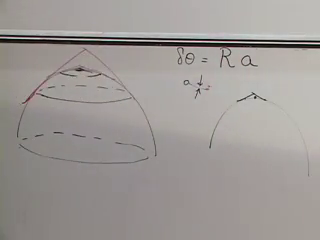
\includegraphics[width=0.90\textwidth]{lecture_06_figure_16.png}
  \caption{The local two-dimensional law written on the board as
  \(\delta\theta=R a\): holonomy angle equals curvature times a small
  enclosed area.}
  \lectureframe{01:25:30}
\end{figure}

\begin{classroomqa}
\audiencequestion{Must the small loop be circular, and should its area be
measured on the surface or in a projection?
\lecturetimestamp{01:24:45--01:26:51}}
\lecturerresponse{The leading term depends on the oriented surface area,
not on the detailed shape of a sufficiently small loop. Surface area is
the intrinsic choice. At infinitesimal scale it differs from a tangent
plane projection only at higher order, which is why the distinction does
not affect Eq.~\eqref{eq:l06-small-loop-curvature}.}
\end{classroomqa}

\begin{classroomqa}
\audiencequestion{For an embedded sphere, do the transported vectors lie
on the curved surface or in the surrounding three-dimensional space?
\lecturetimestamp{01:26:52--01:28:11}}
\lecturerresponse{A vector at \(p\) belongs to the intrinsic tangent space
\(T_pM\). In an embedding picture that tangent space is represented by the
plane tangent to the sphere at \(p\); the vector need not be the tangent
of the particular curve being followed. As the base point moves, the
tangent plane changes.}
\end{classroomqa}

\begin{classroomqa}
\audiencequestion{What happens for a large loop such as the equator,
where the small-area formula is no longer valid?
\lecturetimestamp{01:28:11--01:28:35}}
\lecturerresponse{One integrates the curvature over the enclosed region:
\(\Delta\alpha=\int_\Sigma K\,dA\), with the angle understood modulo
\(2\pi\) and with the appropriate orientation. The equator bounds a
hemisphere whose integrated curvature is \(2\pi\), so a vector can return
visibly unchanged without contradicting the nonzero curvature.}
\end{classroomqa}

\section{Topology and the Torus}

Finite-loop holonomy can reveal topology as well as local curvature. The
flat M\"obius band is nonorientable. The flat torus is different: identify
opposite sides of a Euclidean rectangle by translations,
\begin{equation}
  (x,y)\sim(x+L_x,y),
  \qquad
  (x,y)\sim(x,y+L_y).
  \label{eq:l06-flat-torus}
\end{equation}
The quotient is intrinsically flat even though it cannot be drawn as the
usual smooth doughnut in three-dimensional Euclidean space without
distorting distances.

\begin{figure}[tbp]
  \centering
  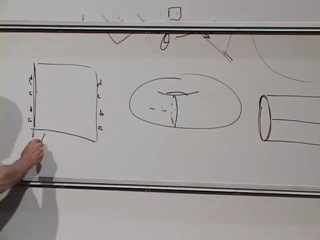
\includegraphics[width=0.90\textwidth]{lecture_06_figure_17.png}
  \caption{The torus as a rectangle with opposite edges identified,
  contrasted with cylinder and doughnut pictures. The quotient metric can
  be flat even though the familiar embedding is curved.}
  \lectureframe{01:33:00}
\end{figure}

The familiar embedded torus has positive Gaussian curvature on its outer
side and negative curvature near the inner rim. Its total Gaussian
curvature is zero:
\begin{equation}
  \int_{\mathbb T^2}K\,dA=0.
  \label{eq:l06-torus-gauss-bonnet}
\end{equation}
This is the torus case of the Gauss--Bonnet theorem. Zero total curvature
does not mean zero curvature point by point.

\begin{classroomqa}
\audiencequestion{Can the flat rectangular torus be physically folded
into an ordinary doughnut, and what curvature does a real torus have?
\lecturetimestamp{01:30:34--01:36:20}}
\lecturerresponse{The rectangle with translated edge identifications is
an abstract flat torus. A smooth isometric embedding of that flat metric
does not exist in ordinary three-dimensional Euclidean space; folding
paper introduces creases or stretching. It can be embedded smoothly in
higher dimension. The standard doughnut in three dimensions is not flat:
its outer region has positive curvature, its inner region negative
curvature, and the integral cancels to zero.}
\end{classroomqa}

\section{The Sign of Curvature}

Give the boundary of a small area an orientation. Call counterclockwise
positive and clockwise negative. Once a convention for vector rotation is
fixed, positive curvature means that the holonomy rotation and the
oriented area have the same sign; negative curvature means they have
opposite signs.

\begin{figure}[tbp]
  \centering
  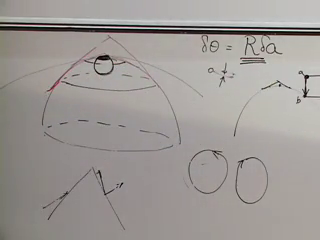
\includegraphics[width=0.89\textwidth]{lecture_06_figure_18.png}
  \caption{Oriented loops and vector rotations used to assign a sign to
  the two-dimensional curvature coefficient.}
  \lectureframe{01:39:45}
\end{figure}

Removing a wedge creates positive concentrated curvature at the cone tip.
The complementary construction is to cut the sheet and insert an extra
wedge, producing an angular excess. A vector transported counterclockwise
then rotates in the opposite direction. This is a concentrated model of
negative curvature.

Smooth negative curvature has the local shape of a saddle rather than a
sphere.

\begin{figure}[tbp]
  \centering
  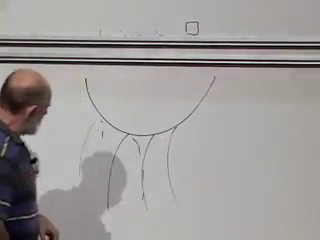
\includegraphics[width=0.80\textwidth]{lecture_06_figure_19.png}
  \caption{A saddle-shaped patch, the characteristic local picture of
  negative Gaussian curvature.}
  \lectureframe{01:40:30}
\end{figure}

The embedded torus exhibits both signs on one connected surface. Its
sphere-like exterior is positively curved; the saddle-like region near
the hole is negatively curved.

\begin{figure}[tbp]
  \centering
  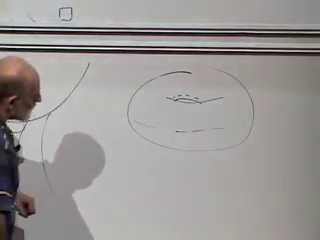
\includegraphics[width=0.82\textwidth]{lecture_06_figure_20.png}
  \caption{The torus cross-section used to distinguish the positively
  curved outer region from the negatively curved inner region.}
  \lectureframe{01:43:45}
\end{figure}

\begin{classroomqa}
\audiencequestion{If small loops are drawn at different places on a real
torus, do they all give the same curvature?
\lecturetimestamp{01:35:25--01:36:20}}
\lecturerresponse{No. The coefficient \(K(p)\) varies over the embedded
torus. It is positive outside, negative inside, and passes through zero
between those regions. Only its integral over the whole torus vanishes.}
\end{classroomqa}

\section{Back to Space-Time and Gravity}

Everything we have done has a space-time counterpart. Replace the
positive-definite spatial metric by a Lorentzian metric, transport
four-vectors with its Levi--Civita connection, and examine what happens
around small loops in different coordinate planes. In more than two
dimensions both the plane of the loop and the plane in which the vector
rotates matter. The object encoding all of those possibilities is the
Riemann curvature tensor, which is the subject of the next lecture.

The physical program of general relativity can now be stated without yet
writing its field equation:
\begin{equation}
  \text{energy and momentum}
  \longrightarrow
  \text{space-time curvature}
  \longrightarrow
  \text{geodesic motion}.
  \label{eq:l06-gr-program}
\end{equation}
Mass is one form of energy, and energy and momentum together source the
curvature that cannot be removed by an accelerated frame throughout a
region. Freely falling particles follow space-time geodesics. In the
weak-field, slow-motion limit those geodesics reproduce Newtonian
trajectories, with relativistic corrections. The Schwarzschild geometry
will provide the central example.

\begin{classroomqa}
\audiencequestion{If a curved surface is embedded in a flat
higher-dimensional space, is intrinsic parallel transport just keeping
the vector parallel in the embedding space?
\lecturetimestamp{01:48:54--01:51:33}}
\lecturerresponse{No. Keeping an ambient vector fixed would generally
make it leave the surface's tangent plane. Intrinsic Levi--Civita
transport keeps the vector tangent and removes only the tangent component
of its change. In an embedding picture, one may differentiate in the
ambient space and project back onto the changing tangent plane. The
definition itself needs only the metric on the surface, not the
embedding.}
\end{classroomqa}

The central lesson is therefore local but powerful. At every regular event
we can choose a freely falling frame in which the connection vanishes.
After moving around a loop, those local frames need not fit back together.
That mismatch is curvature, and in general relativity it is the invariant
content of the gravitational field.
